\documentclass[dvipsnames]{beamer}
%Text
\usepackage[utf8]{inputenc}
\usepackage[english]{babel}
\usepackage{xcolor}
%Theme
\usetheme[pageofpages=of,% String used between current and total page counts
          bullet=circle,% Use circles instead of squares for bullets.
          titleline=true,% Show a line below the frame title.
          alternativetitlepage=true,% Use the fancy title page.
          titlepagelogo=mcmaster_logo,% Logo for the first page.
          watermark=mcmaster_logo,% Watermark used in every page.
          watermarkheight=1px,% Height of the watermark.
          watermarkheightmult=1,%watermakr x bigger than watermarkheight
          ]{Torino}
%Graphics
\usepackage{graphicx}
\graphicspath{{./pics/}}
\usepackage[section]{placeins} %for FloatBarrier
%Refernces
\usepackage{appendixnumberbeamer}
\usepackage[natbib=true,
            bibencoding=utf8,
            style=numeric,
            backend=biber,
            autocite=superscript,
            sorting=none,
            useprefix=true]{biblatex}
\addbibresource{../refs.bib}
\usepackage[absolute,overlay]{textpos}
%Tikz
\usepackage{tikz}% for flow chart
\usepackage{moresize} %for ssmall font size
\usetikzlibrary{shapes,arrows,positioning,fit,quotes,shapes.misc}% for flow chart
%Styles
\tikzstyle{block} = [circle,
                     fill=green!20,
                     text centered,
                     font=\ssmall,
                     text width=1.5cm,
                     rounded corners,
                     draw]
\tikzstyle{slock} = [circle,
                     fill=red!20,
                     font=\ssmall,
                     text width=1.5cm,
                     text centered,
                     rounded corners,
                     draw]
\tikzstyle{flock} = [circle,
                     fill=blue!20,
                     font=\ssmall,
                     text width=1.5cm,
                     text centered,
                     rounded corners,
                     draw]
\tikzstyle{line} = [draw, -latex']
\newcommand{\Checkmark}{$\mathbin{\tikz [x=2.4ex, y=2.4ex, line width=.2ex, green] \draw (0,1) -- (1,0) -- (3,3);}$}
%Abbreviations
\usepackage{acro}
%otu
\DeclareAcronym{otu}{
    short = OTU,
    long  = Operation Taxonomic Unit
}
%pa
\DeclareAcronym{pa}{
    short = P/A,
    long  = Presence/Absence,
}
%mge
\DeclareAcronym{mge}{
    short = MGE,
    long  = Mobile Genetic Element
}
%ecoli
\DeclareAcronym{ecoli}{
    short = \textit{E. coli},
    long  = \textit{Escherichia coli}
}
%crispr
\DeclareAcronym{cas}{
    short = Cas,
    long  = CRISPR-associated
}
%crispr
\DeclareAcronym{crsp}{
    short = CRISPR,
    long  = Clustered Regularly Interspaced Short Palindromic Repeat
}
%HGT
\DeclareAcronym{hgt}{
    short = HGT,
    long = Horizontal Gene Transfer
}
%Title
\title{The Effects Of CRISPR-Cas Systems On\newline
        The Rate Of Horizontal Gene Transfer}
\subtitle{\vspace{0.1in} A Network Theoretic Approach}
\date{\today}
\author{Siddharth Reed\\
        Undergraduate Thesis}
\institute{Golding Lab,\\
           Biology Department,\\
           McMaster University
}
\begin{document}
\watermarkoff %theme has watermark on every slide, turning that off
%Title Slide
\begin{frame}[t,plain]
    \titlepage
\end{frame}
%Table Of Contents
\begin{frame}{Table of Contents}
  \setbeamertemplate{section in toc}[sections numbered]
  \tableofcontents[hideallsubsections]
\end{frame}
\section{CRISPR-Cas systems}
\begin{frame}[fragile,noframenumbering]{}
    \begin{center}
        \Huge \textcolor{OliveGreen}{CRISPR-Cas systems}
    \end{center}
\end{frame}
\begin{frame}[fragile]{What Are They?}
    \begin{columns}
    \begin{column}{0.5\textwidth}
        \begin{itemize}
            \item<2-> Adaptive Bacterial Immune System
            \item<3-> Protects against foreign DNA
            \item<4-> Requires Cas proteins and CRISPR loci
        \end{itemize}
    \end{column}
    \begin{column}{0.5\textwidth}
        \begin{figure}[htb!]\onslide<2->
            \makebox[\textwidth][c]{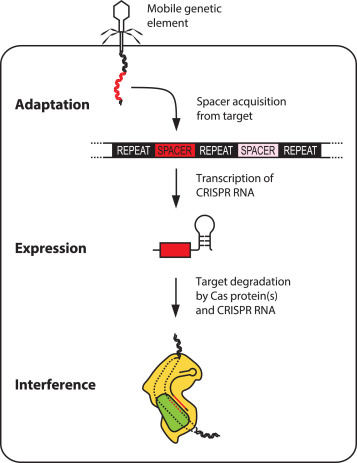
\includegraphics[width=0.8\linewidth]{CRISPR-immunity_crispgen.jpg}}
            \autocite{crispgen}
        \end{figure}
    \end{column}
    \end{columns}
\end{frame}
\begin{frame}[fragile]{Diversity \& Ubiquity}
    \begin{columns}
    \begin{column}{0.5\textwidth}
        \begin{itemize}
            \item<2-> $45\%$ of bacteria have CRISPR loci $(n=6782)$\autocite{crispdb}
            \item<3-> 3 Main Types, multiple subtypes\autocite{acqorres}
            \item<4-> CRISPR arrays represent unique life history of an organism
            \item<5-> $11\%-28\%$ are false or orphaned CRISPR loci\autocite{ineqcas}
        \end{itemize}
    \end{column}
    \begin{column}{0.5\textwidth}
    \begin{figure}[htb!]\onslide<2->
        \makebox[\textwidth][c]{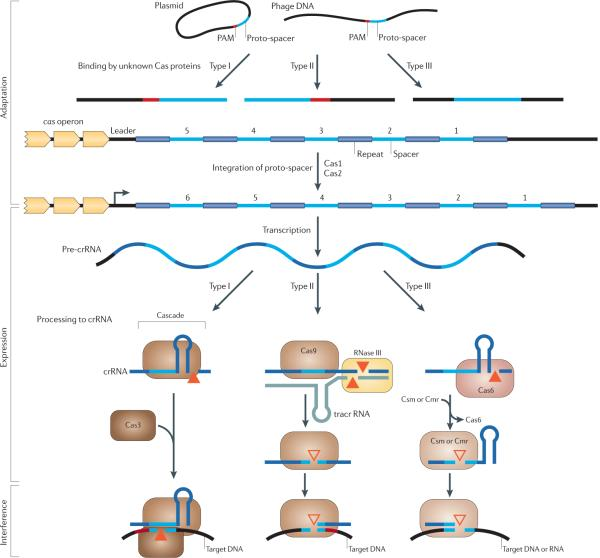
\includegraphics[width=0.9\linewidth]{CRISPR-types_evocas.jpg}}
        \autocite{evocas}
    \end{figure}
    \end{column}
    \end{columns}
\end{frame}
\begin{frame}[fragile]{Biotech Application}
        \begin{figure}[htb!]\onslide<2->
            \makebox[\textwidth][c]{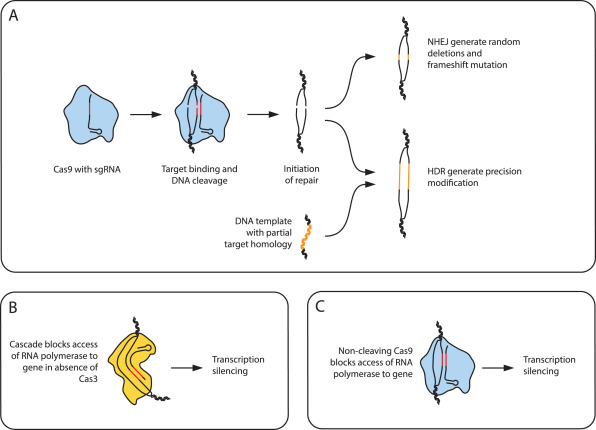
\includegraphics[width=0.8\linewidth]{CRISPR-apps.jpg}}
            \autocite{crispgen}
        \end{figure}
\end{frame}
\section{Horizontal Gene Transfer}
\begin{frame}[fragile,noframenumbering]{}
    \begin{center}
        \Huge \textcolor{OliveGreen}{Horizontal Gene Transfer}
    \end{center}
\end{frame}
\begin{frame}[fragile]{Mechanisms}
    \begin{columns}
    \begin{column}{0.5\textwidth}
        \begin{figure}[htb!]\onslide<1->
            \makebox[\textwidth][c]{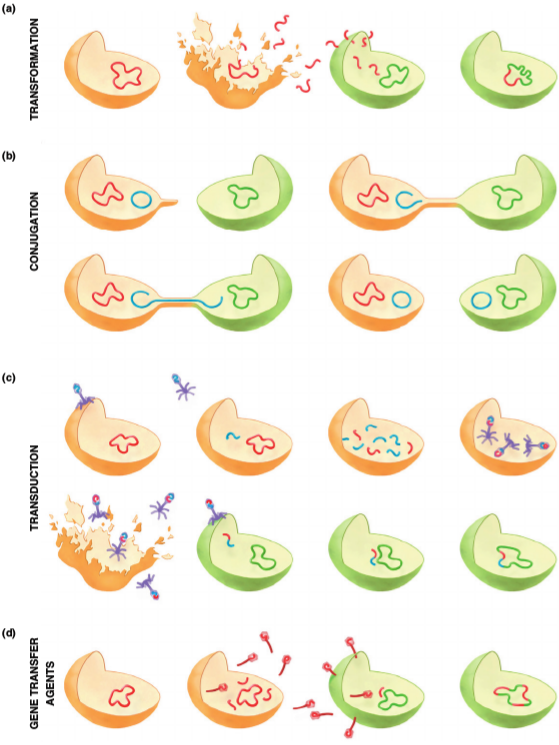
\includegraphics[width=0.8\linewidth]{hgt_mechanisims_trendslgt.png}}
            \autocite{trendslgt}
        \end{figure}
    \end{column}
    \begin{column}{0.5\textwidth}
        \begin{itemize}
            \item<2-> Conjugation: Transfer of DNA through cell-cell connections\autocite{trendslgt}
            \item<3-> Transformation: Incorportaion of free-floating DNA into the genome\autocite{trendslgt}
            \item<4-> Transduction: Transfer of DNA through phage\autocite{trendslgt}
            \item<5-> \textbf{CRISPR-Cas directly affects Transduction and Transformation}\autocite{trendslgt}
        \end{itemize}
    \end{column}
    \end{columns}
\end{frame}
\begin{frame}[fragile]{Pan-Genomes}
\begin{columns}
    \begin{column}{0.5\textwidth}
        \begin{figure}[htb!]\onslide<2->
            \makebox[\textwidth][c]{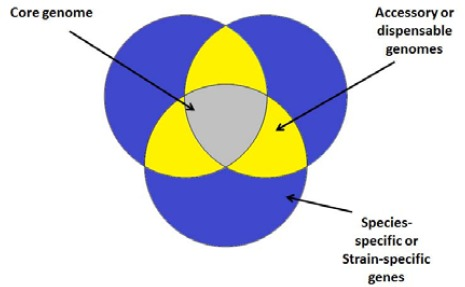
\includegraphics[width=\linewidth]{pangenome_pang.jpg}}
            \autocite{pang}
        \end{figure}
    \end{column}
    \begin{column}{0.5\textwidth}
        \begin{figure}[htb!]\onslide<3->
            \makebox[\textwidth][c]{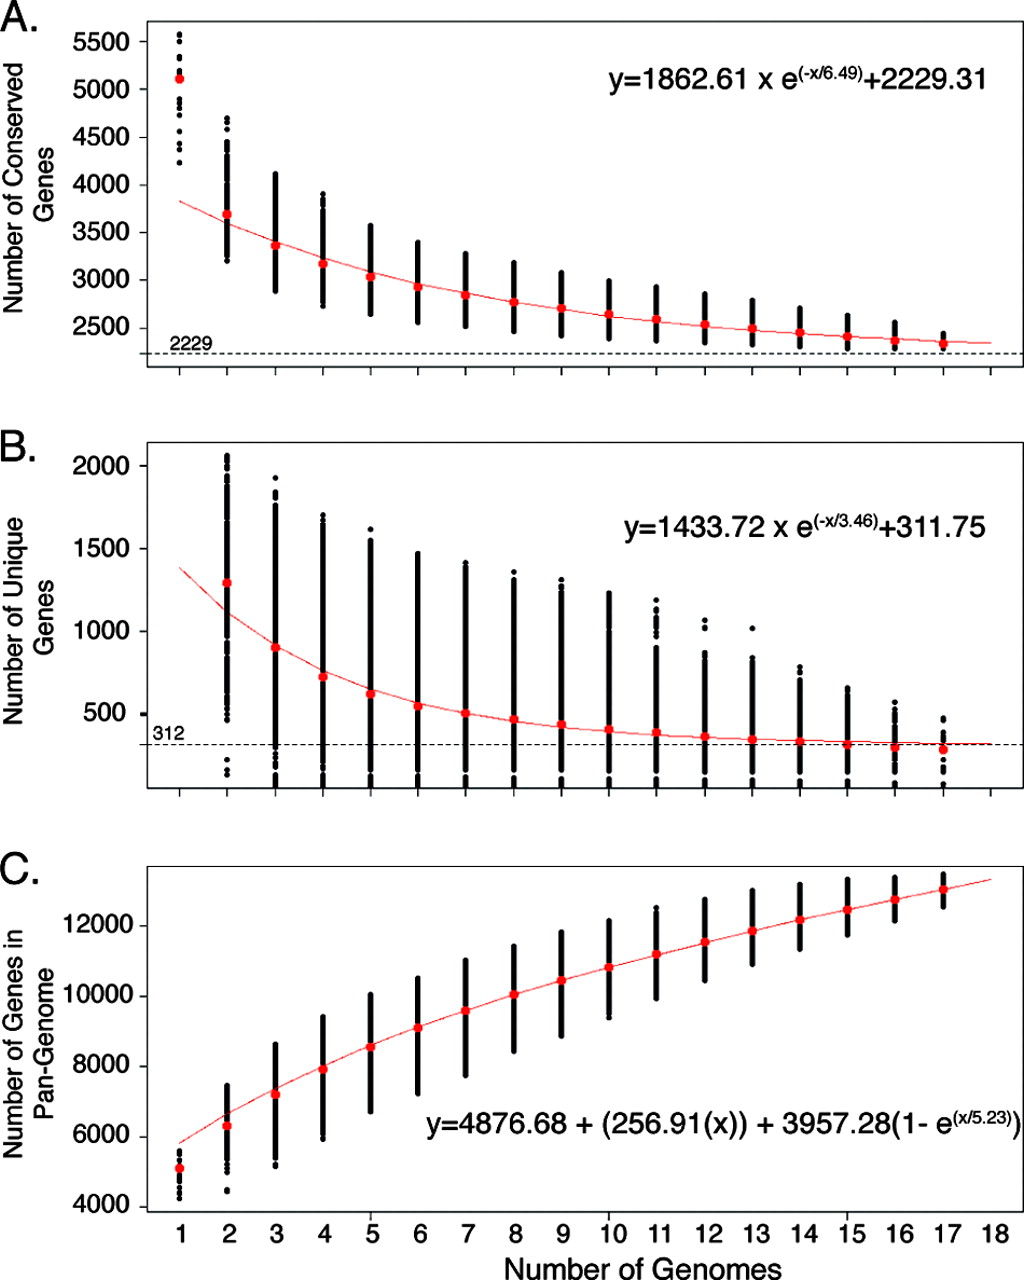
\includegraphics[width=0.8\linewidth]{pangGrapgs_ecopan.jpg}}
            \autocite{ecopan}
        \end{figure}
    \end{column}
\end{columns}
\end{frame}
\begin{frame}[fragile]{Rate Influencing Factors}
    \begin{itemize}
        \item<2-> Amount of exogenous DNA/cell density/phage density
        \item<3-> Selective pressures
        \item<4-> Metabolic costs
        \item<5-> Sequence compatibility
    \end{itemize}
\end{frame}
\begin{frame}[fragile]{Applications}
    \begin{figure}[htb!]\onslide<2->
        \makebox[\textwidth][c]{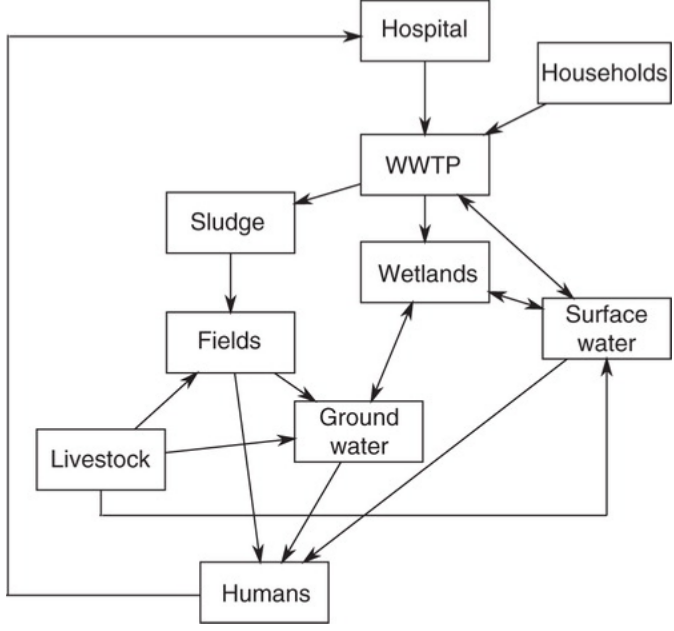
\includegraphics[width=0.6\linewidth]{spreadDiagram_argspread.png}}
        \autocite{argspread}
    \end{figure}
\end{frame}
\section{Phylogenomic Networks}
\begin{frame}[fragile,noframenumbering]{}
    \begin{center}
        \Huge \textcolor{OliveGreen}{Phylogenomic Networks}
    \end{center}
\end{frame}
\begin{frame}[fragile]{What is A Network?}
\begin{columns}
    \begin{column}{0.5\textwidth}
        \begin{figure}[htb!]\onslide<2->
            \makebox[\textwidth][c]{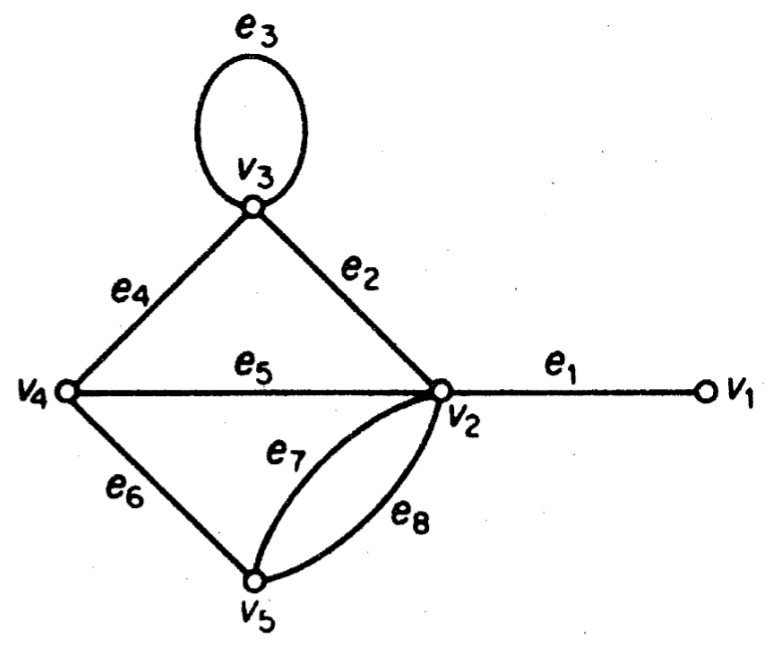
\includegraphics[width=0.8\linewidth]{graphExample_bondy.png}}
        \end{figure}
        \autocite{bondy}
    \end{column}
    \begin{column}{0.5\textwidth}
        \begin{itemize}
            \item<2-> Useful mathematical abstraction of real world system
            \item<3-> Nodes can have attributes
            \item<4-> Directed or Undirected Edges
            \item<5-> Weighted or Unweighted Edges
        \end{itemize}
    \end{column}
\end{columns}
\end{frame}
\begin{frame}[fragile]{Prokaryotic ``Net of Life''}
    \begin{figure}[htb!]\onslide<2->
        \makebox[\textwidth][c]{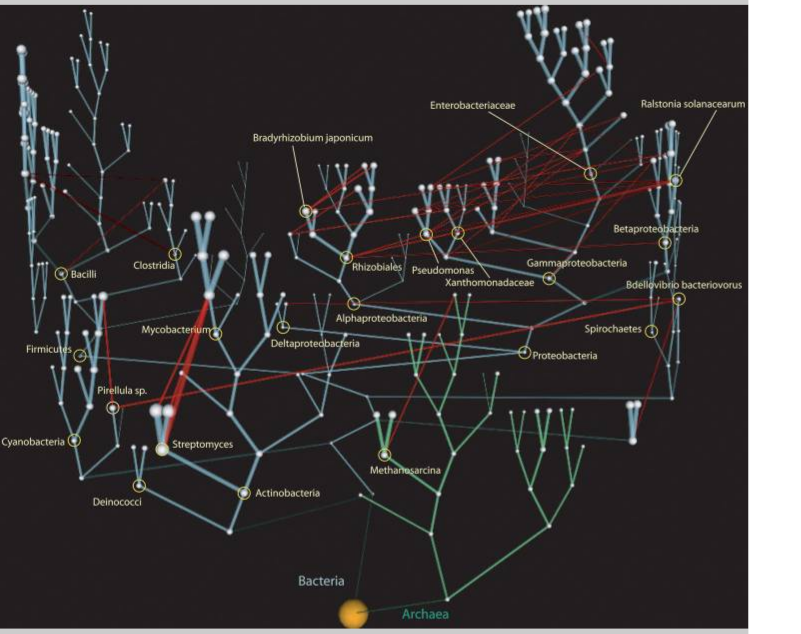
\includegraphics[width=0.7\linewidth]{net_netoflife.png}}
        \autocite{netoflife}
    \end{figure}
\end{frame}
\begin{frame}[fragile]{Construction}
        \begin{figure}[htb!]\onslide<1->
            \makebox[\textwidth][c]{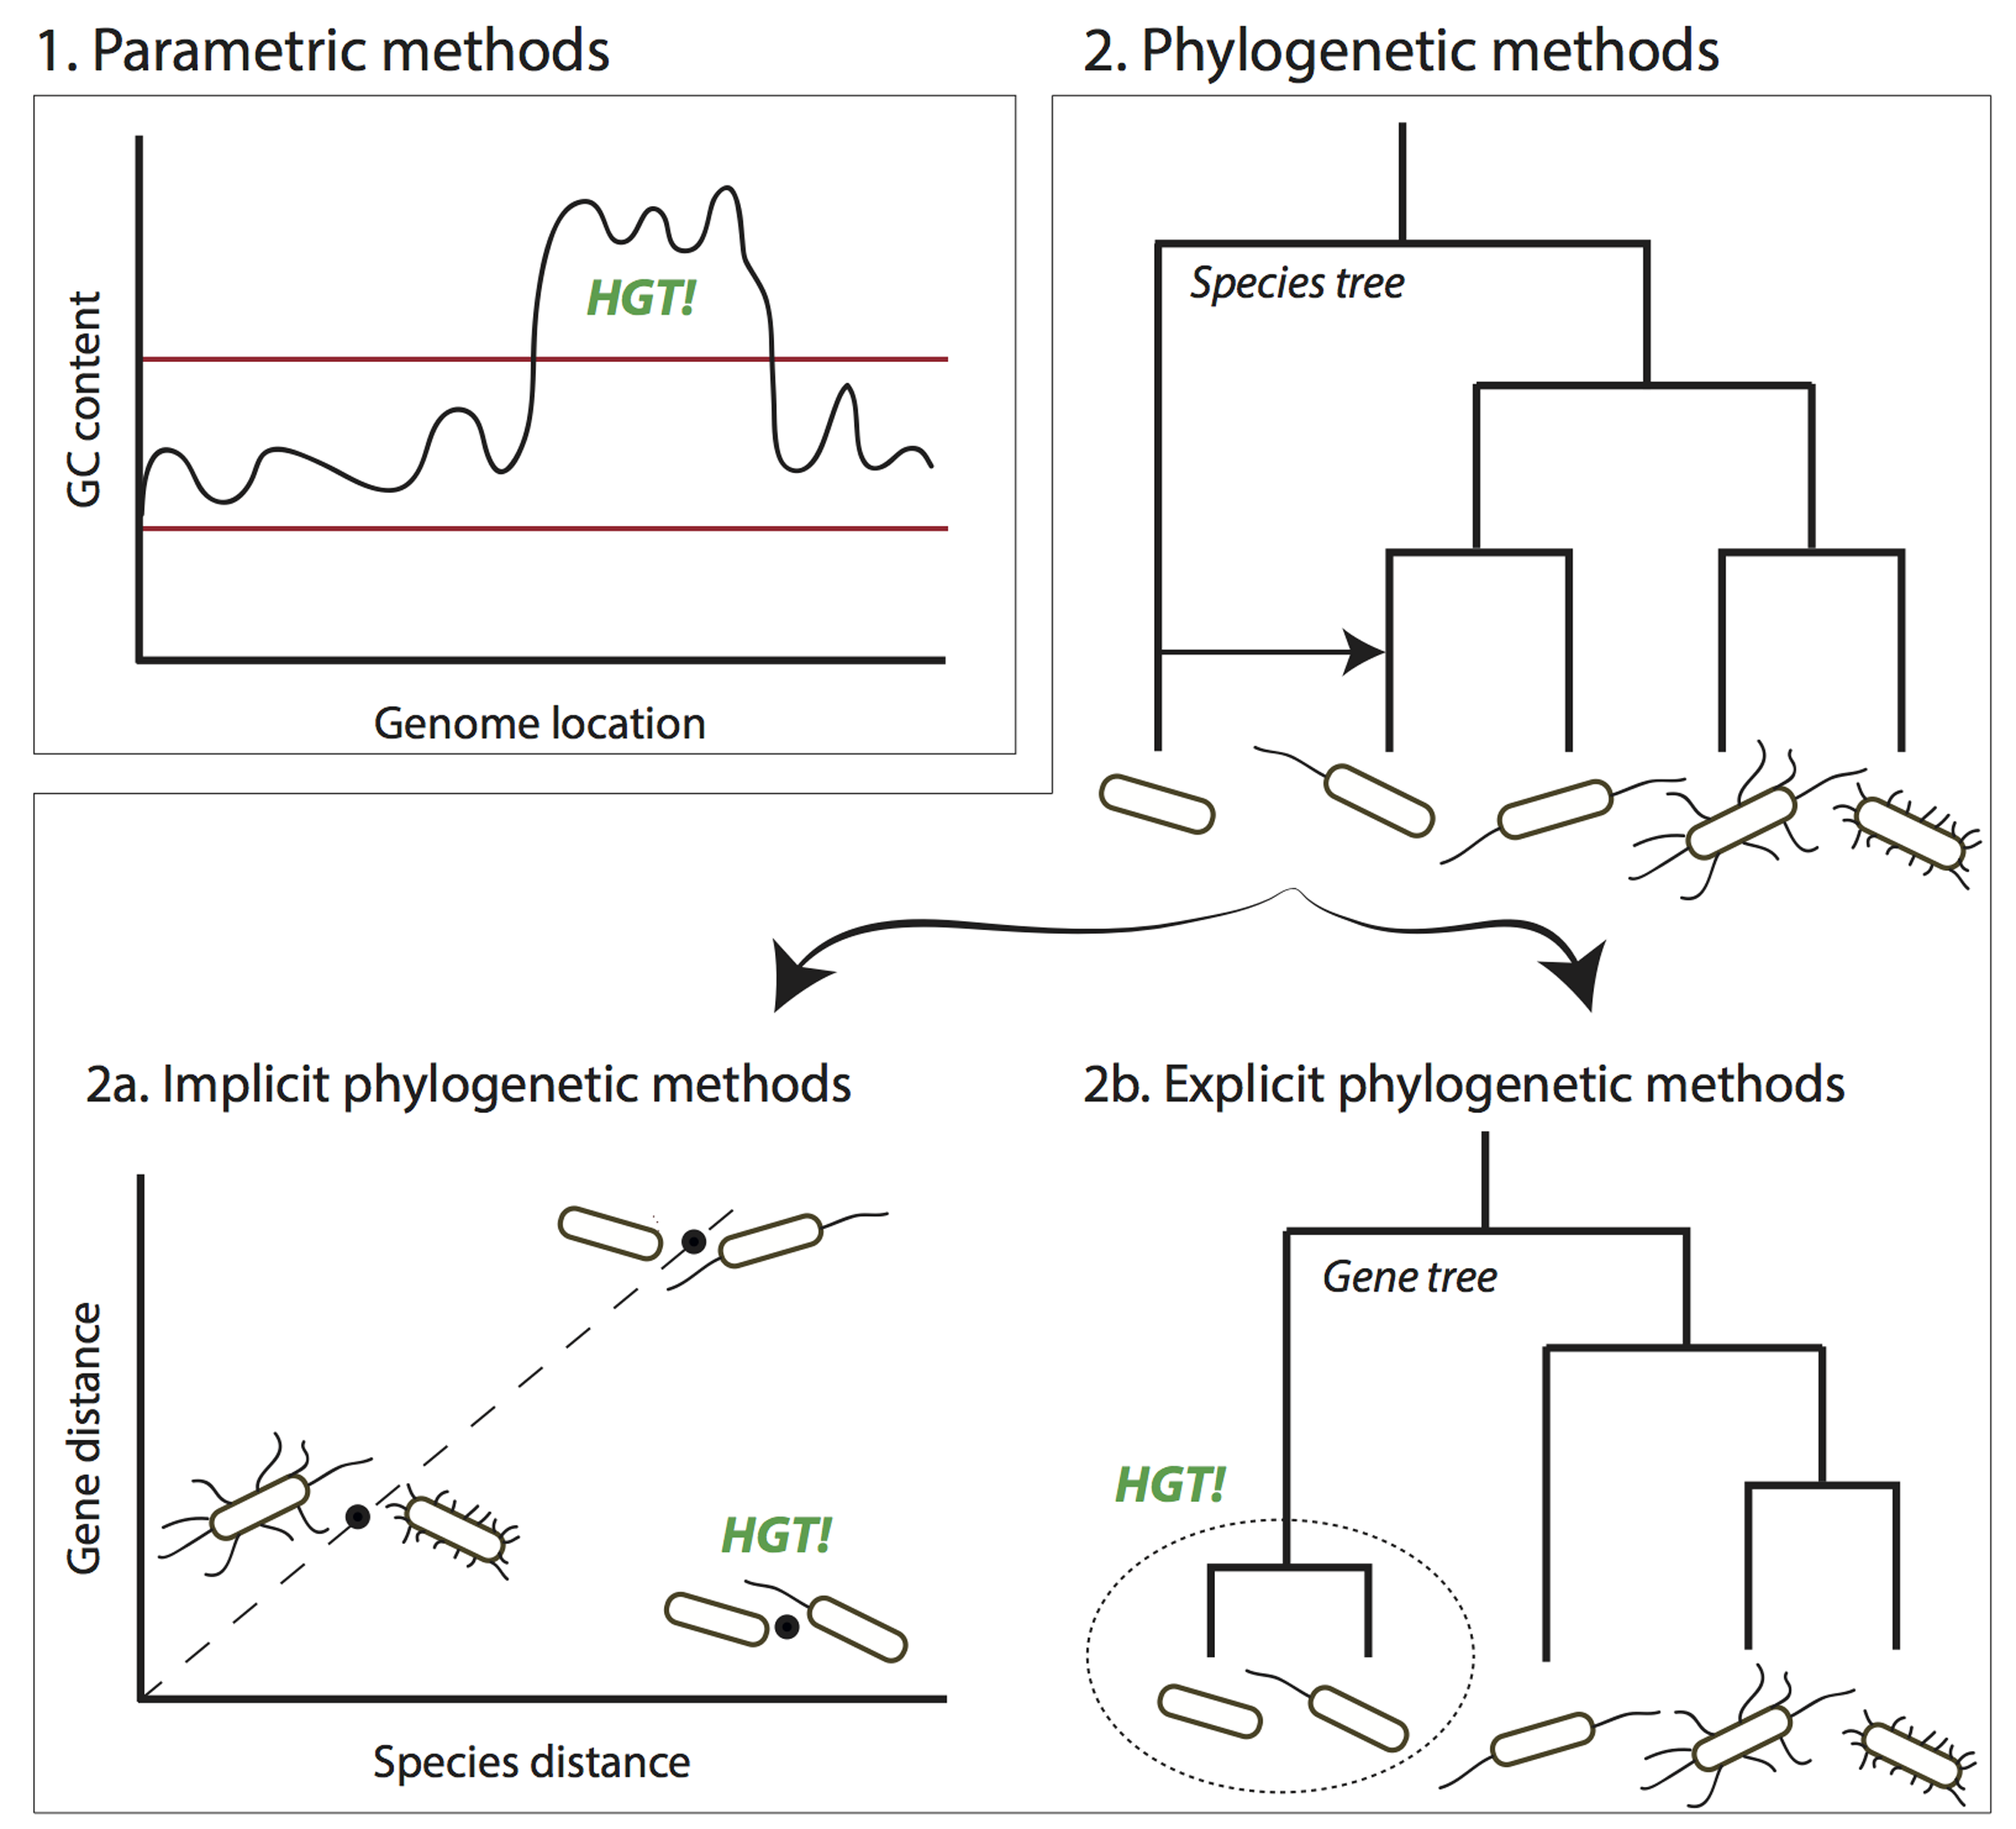
\includegraphics[width=0.6\linewidth]{hgtiInferenceMethods_ihgt.png}}
            \autocite{ihgt}
        \end{figure}
\end{frame}
\section{Do CRRISPR Systems Affect Horizontal Gene Transfer?}
\begin{frame}[fragile,noframenumbering]{}
    \begin{center}
        \Huge \textcolor{OliveGreen}{Do CRRISPR Systems Affect Horizontal Gene Transfer?}
    \end{center}
\end{frame}
\begin{frame}[fragile,noframenumbering]{}
    \begin{center}
        \Huge Yes
    \end{center}
\end{frame}
\begin{frame}[fragile]{CRISPR Cost Complexity}
    \begin{itemize}
        \item<2-> Cost tradeoff factors:
        \begin{itemize}
            \item<3-> Metabolic maintenace\autocite{crispgen}
            \item<4-> Environmental pressures\autocite{hospital}
            \item<5-> Off-target effects (autoimmune)\autocite{selfcrisp}
            \item<6-> Anti-CRISPR systems\autocite{acqorres}
            \item<7-> Phage virulence/density\autocite{acqorres}
            \item<8-> Prophage abundance\autocite{transhgt}
        \end{itemize}
    \end{itemize}
\end{frame}
\begin{frame}[fragile]{Curbing CRISPR Cost}
    \begin{itemize}
        \item<2-> CRISPRs themselves can be transfered $\implies$ population level immunity\autocite{crisprlgt}
        \item<3-> Selective CRISPR inactivation\autocite{crispgen}
        \item<4-> CRISPR can enhance transduction-mediated HGT\autocite{transhgt}
    \end{itemize}
\end{frame}
\begin{frame}[fragile]{Previous Findings}
    \begin{itemize}
        \item<2-> Gophna et al. (2015) found that CRISPR has no effect on HGT over short evolutionary timescales\autocite{gophna15}
        \begin{itemize}
            \item<3-> Assume all singletons arrose from HGT
            \item<4-> Used GC\% to identify HGT
        \end{itemize}
        \item<5-> Contradicted by a former thesis student
        \begin{itemize}
            \item<6-> Can see inhibitory effects of CRIPSR on HGT over short evolutionary time scales
            \item<7-> Higher gene indel rates for CRISPR containg genera than non-CRISPR containing outgroups
        \end{itemize}
    \end{itemize}
\end{frame}
\section{My Project}
\begin{frame}[fragile]{}
    \begin{center}
        \Huge \textcolor{OliveGreen}{My Project}
    \end{center}
\end{frame}
\begin{frame}[fragile]{Hypothesis}
    \onslide<1-> \begin{block}{Null Hypothesis}
     Bacterial strains or genera with known CRISPR systems will show no significant differences in network statistics compared to those strains or genera without known CRISPR systems\onslide<1>.
    \end{block}
    \onslide<2-> \begin{block}{Alternative Hypothesis}
     Bacterial strains or genera with known \ac{crsp} systems will show a significant difference in at least 1 network statistic compared to those strains or  genera without known \ac{crsp} systems.\onslide<2>
    \end{block}
\end{frame}
\begin{frame}[fragile]{Objectives}
    \onslide<2-> \begin{block}{Within Network Comparisons}
        For genera with CRISPR conatining strains, compare the node statistics of CRIPSR-containing strain to non-CRISPR-containing strains.
    \end{block}
    \onslide<3-> \begin{block}{Between Network Comparisons}
        For genera with no CRISPR conatining strains, compare the network statistics of mixed to non-CRISPR-containing networks.
    \end{block}
    \onslide<4-> \begin{block}{Gene Indel Rates vs. Network Statistics}
        Compare gene InDel rates to node/network statistics for CRISPR-containing and non-CRISPR-containing strains/genera.
    \end{block}
\end{frame}
\begin{frame}[fragile]{Workflow}
\begin{center}
    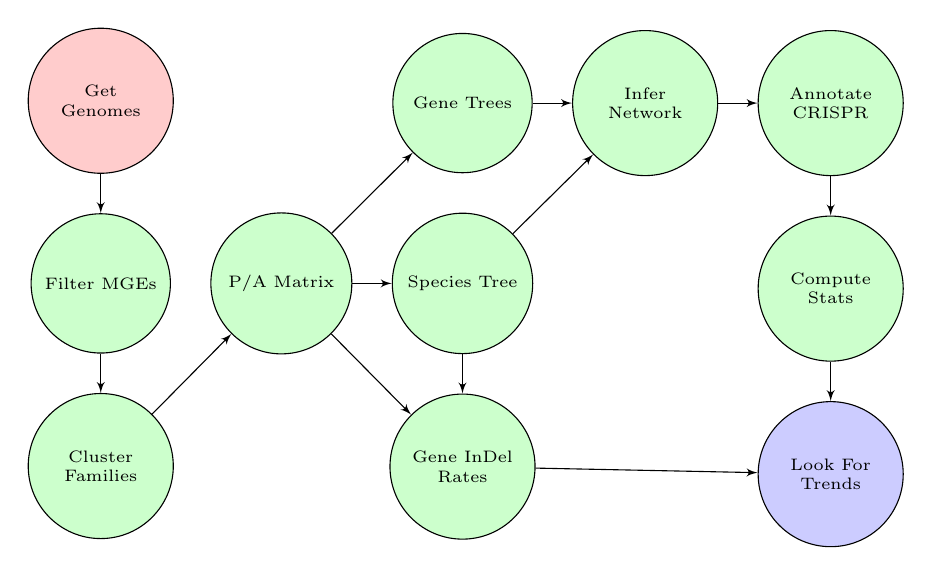
\begin{tikzpicture}
        % boxes
        \node [slock]                       (node1)  {Get Genomes};\onslide<1->
        \node [block,below=0.5cm of node1]  (node2)  {Filter MGEs};\onslide<3->
        \node [block,below=0.5cm of node2]  (node3)  {Cluster Families};\onslide<4->
        \node [block,right=0.5cm of node2]  (node4)  {P/A Matrix};\onslide<5->
        \node [block,right=0.5cm of node4]  (node5)  {Species Tree};\onslide<6->
        \node [block,above=0.5cm of node5]  (node6)  {Gene Trees};\onslide<7->
        \node [block,below=0.5cm of node5]  (node7)  {Gene InDel Rates};\onslide<8->
        \node [block,right=0.5cm of node6]  (node8)  {Infer Network};\onslide<9->
        \node [block,right=0.5cm of node8]  (node9)  {Annotate CRISPR};\onslide<10->
        \node [block,below=0.5cm of node9]  (node10) {Compute Stats};\onslide<11->
        \node [flock,below=0.5cm of node10] (node11) {Look For Trends};\onslide<12->
        %lines
        \path [line] (node1) -- (node2);\onslide<2->
        \path [line] (node2) -- (node3);\onslide<3->
        \path [line] (node3) -- (node4);\onslide<4->
        \path [line] (node4) -- (node5);\onslide<5->
        \path [line] (node4) -- (node7);\onslide<6->
        \path [line] (node5) -- (node7);\onslide<6->
        \path [line] (node4) -- (node6);\onslide<7->
        \path [line] (node5) -- (node8);\onslide<8->
        \path [line] (node6) -- (node8);\onslide<8->
        \path [line] (node8) -- (node9);\onslide<9->
        \path [line] (node9) -- (node10);\onslide<10->
        \path [line] (node7) -- (node11);\onslide<11->
        \path [line] (node10) -- (node11);\onslide<11->
    \end{tikzpicture}
\end{center}
\end{frame}
\begin{frame}[fragile]{Network Statistics}
    \begin{itemize}
        \item<2-> \textbf{Total/Average edge weight}: $\sum_i w_i$,$\frac{\sum_i w_i}{N}$
        \item<3-> \textbf{Network Density}: $\frac{2E}{N(N-1)}$
        \item<4-> \textbf{Network Diameter}: The shortest path between the 2 furthest nodes.
        \item<5-> \textbf{Node Closeness Centrality}: $\frac{N-1}{\sum_v d(u,v)}$ where $d(x,y)$ is the shortest path $v \to u$.
        \item<6-> \textbf{Node Clustering Coefficient}: $\frac{2e}{k(k-1)}$ where $k$ is the neighbors and $e$ is the edges between all neighbors.
        \item<7-> \textbf{Edge Weight KL Divergence}: $D_{KL}(P||Q)= \int_{-\infty}^{\infty} p(x)log(\frac{p(x)}{q(x)}dx$
        \item<8-> \textbf{Node Associativity}: $\frac{j(j+1)(\overline{k}-\mu_q)}{2E\sigma^2_q}$ where $j$ is the excess degree of the node and $\overline{k}$ is the average excess degree of the node's neighbors and $\mu_q$ and $\sigma_q$ are the mean and standard variation of the excess degree distribution.
    \end{itemize}
\end{frame}
\begin{frame}[fragile,noframenumbering]{Thanks}
    Thank you to
    \begin{itemize}
        \item Dr. G. Brian Golding
        \item The Golding lab
            \begin{itemize}
                \item Caitlin Simopoulos
                \item Daniella Lato
                \item Zachery Dickson
                \item Sam Long
                \item Lucy Zhang
                \item Brianne Laverty
                \item Nicole Zhang
            \end{itemize}
        \item Everyone here for listening
    \end{itemize}
\end{frame}
\begin{frame}[allowframebreaks,noframenumbering]{References}
    \printbibliography
\end{frame}
\end{document}

